% Use the ijcai22 format

%%%% ijcai22.tex

\typeout{IJCAI--22 Instructions for Authors}

% These are the instructions for authors for IJCAI-22.

\documentclass{article}
\pdfpagewidth=8.5in
\pdfpageheight=11in
% The file ijcai22.sty is NOT the same as previous years'
\usepackage{ijcai22}

% Use the postscript times font!
\usepackage{times}
\usepackage{soul}
\usepackage{url}
\usepackage[hidelinks]{hyperref}
\usepackage[utf8]{inputenc}
\usepackage[small]{caption}
\usepackage{graphicx}
\usepackage{amsmath}
\usepackage{amsthm}
\usepackage{booktabs}
\usepackage{algorithm}
\usepackage{algorithmic}
\usepackage{tkz-graph}

\urlstyle{same}

% the following package is optional:
%\usepackage{latexsym}

% See https://www.overleaf.com/learn/latex/theorems_and_proofs
% for a nice explanation of how to define new theorems, but keep
% in mind that the amsthm package is already included in this
% template and that you must *not* alter the styling.
\newtheorem{example}{Example}
\newtheorem{theorem}{Theorem}

\newtheorem{definition}{Definition}
\newtheorem{proposition}{Proposition}

% Following comment is from ijcai97-submit.tex:
% The preparation of these files was supported by Schlumberger Palo Alto
% Research, AT\&T Bell Laboratories, and Morgan Kaufmann Publishers.
% Shirley Jowell, of Morgan Kaufmann Publishers, and Peter F.
% Patel-Schneider, of AT\&T Bell Laboratories collaborated on their
% preparation.

% These instructions can be modified and used in other conferences as long
% as credit to the authors and supporting agencies is retained, this notice
% is not changed, and further modification or reuse is not restricted.
% Neither Shirley Jowell nor Peter F. Patel-Schneider can be listed as
% contacts for providing assistance without their prior permission.

% To use for other conferences, change references to files and the
% conference appropriate and use other authors, contacts, publishers, and
% organizations.
% Also change the deadline and address for returning papers and the length and
% page charge instructions.
% Put where the files are available in the appropriate places.

% PDF Info Is REQUIRED.
% Please **do not** include Title and Author information
\pdfinfo{
	/TemplateVersion (IJCAI.2022.0)
}

\title{Bayesian Networks and Graph Rewrites}

% Single author syntax
\author{
	Adam Chen
	\affiliations
	Stevens Institute of Technology
	\emails
	achen19@stevens.edu
}



\begin{document}
	
	\maketitle
	
	\begin{abstract}
		Abstract here.
	\end{abstract}
	
		
	\section{Introduction}
	\subsection{Motivating Example}
	$A \rightarrow B \rightarrow C$ is indistinguishable from $C \rightarrow B \rightarrow A$. However, substituting one structure with another in all cases may not preserve validity of a Bayesian network.
	\begin{figure}[b]
	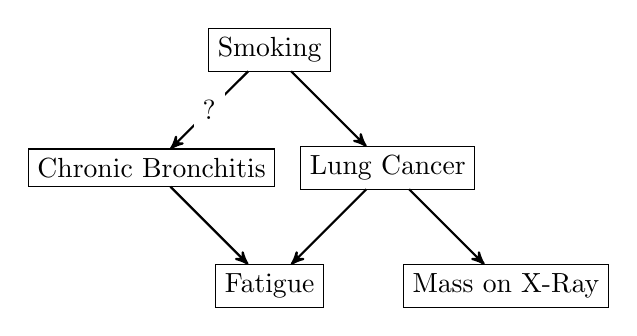
\begin{tikzpicture}[scale=1]
		\tikzstyle{VertexStyle} = [shape=rectangle,minimum width=6ex, draw]
		\tikzstyle{EdgeStyle}   = [->,>=stealth']
		
		\SetGraphUnit{1.5}
		\Vertex{Smoking}  \SOWE(Smoking){Chronic Bronchitis} \SOEA(Smoking){Lung Cancer}
		\SOEA(Chronic Bronchitis){Fatigue} \SOEA(Lung Cancer){Mass on X-Ray}
		\Edge[label=?](Smoking)(Chronic Bronchitis) \Edge(Smoking)(Lung Cancer)
		\Edge(Lung Cancer)(Fatigue) \Edge(Lung Cancer)(Mass on X-Ray) \Edge(Chronic Bronchitis)(Fatigue)
	\end{tikzpicture}
	\caption{Example of a Bayesian Network. As only conditional probabilities, which are symmetric, are specified, the graph is agnostic to whether the ``?'' edge is in the direction shown or is reversed.}
	\label{dir-ex}
	\end{figure}

	\begin{figure}[b]
	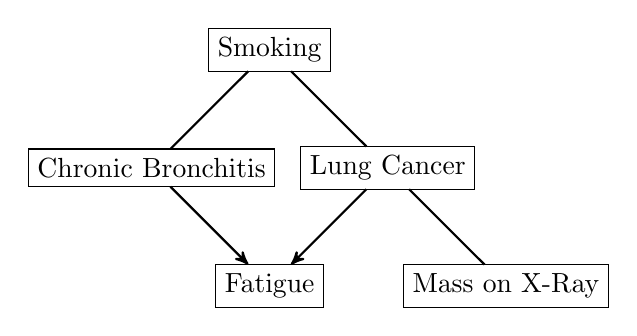
\begin{tikzpicture}[scale=1]
		\tikzstyle{VertexStyle} = [shape=rectangle,minimum width=6ex, draw]
		\tikzstyle{EdgeStyle}   = [-,>=stealth']
		
		\SetGraphUnit{1.5}
		\Vertex{Smoking}  \SOWE(Smoking){Chronic Bronchitis} \SOEA(Smoking){Lung Cancer}
		\SOEA(Chronic Bronchitis){Fatigue} \SOEA(Lung Cancer){Mass on X-Ray}
		\Edge(Smoking)(Chronic Bronchitis) \Edge(Smoking)(Lung Cancer)
		\draw[thick, ->,>=stealth'](Lung Cancer)--(Fatigue); \Edge(Lung Cancer)(Mass on X-Ray) \draw[thick, ->,>=stealth'](Chronic Bronchitis)--(Fatigue);
	\end{tikzpicture}
	\caption{Replacing every undirected edge with an edge in an arbitrary direction, without introducing any new v-structures, yields an equivalent Bayesian Network.}
	\label{undir-ex}
	\end{figure}

	With respect to Figure \ref{undir-ex}, the condition that no cycles and no additional v-structures be introduced limits the choice of direction to four options:
	\begin{enumerate}
		\item The graph as shown in Figure \ref{dir-ex}.
		\item Chronic Bronchitis $\rightarrow$ Smoking $\rightarrow$ Lung Cancer $\rightarrow$ Mass on X-Ray.
		\item Mass on X-Ray $\rightarrow$ Lung Cancer $\rightarrow$ Smoking $\rightarrow$ Chronic Bronchitis.
		\item Chronic Bronchitis $\leftarrow$ Smoking $\leftarrow$ Lung Cancer $\rightarrow$ Mass on X-Ray.
	\end{enumerate}
	Any other choice on arrows would create a new v-structure, either on (Chronic Bronchitis, Smoking, Lung Cancer), or on (Smoking, Lung Cancer, Mass on X-Ray).
	\paragraph{}
	
	We may take a structure $A \rightarrow B$ and replace it with creating a new node $C$ with $A \leftarrow C \rightarrow B$.
	
	\subsection{Divergence of Bayesian Networks from Causality}
	
	\begin{definition}
		Bayesian networks $G_0$ and $G_1$ are isomorphic if $\forall P: G_0$ is compatible with $P \iff G_1$ is compatible with $P$.
	\end{definition}
	
	
	\appendix
	
\end{document}
